\documentclass[a4paper,12pt]{article}

\usepackage[utf8]{inputenc}
\usepackage{polski}
\usepackage[polish]{babel}
\usepackage{graphicx}
\usepackage{url}

\providecommand{\imref}[1]{Rys. \ref{#1}} % referencja do obrazka

%% Define a new 'leo' style for the package that will use a smaller font.
\makeatletter
\def\url@leostyle{%
  \@ifundefined{selectfont}{\def\UrlFont{\sf}}{\def\UrlFont{\small\ttfamily}}}
\makeatother
%% Now actually use the newly defined style.
\urlstyle{leo}

\begin{document}

\author{Jakub Kuźma}
\title{Pioneers - internetowa implementacja gry ,,Osadnicy z Catanu''
  w oparciu o framework Ruby on Rails}
\date{\today}

\begin{titlepage}
\maketitle
\end{titlepage}

\section{Analiza zagadnienia}

\subsection{Osadnicy z Catanu}
Gra planszowa ,,Osadnicy z Catanu'' została stworzona przez
niemieckiego matematyka Klausa Teubera. Po raz pierwszy została ona
wydana w 1995 roku w Niemczech pod nazwą \emph{Die Siedler von
  Catan}. O ogromnej popularności gry na całym świecie może świadczyć
fakt, iż została ona przetłumaczona na ponad 20 języków, w tym język
polski. Na całym świecie organizowane są turnieje gry, a począwszy od
roku 2000 organizowane są coroczne mistrzostwa świata. Pierwsze
polskie wydanie gry przypada na rok 2005. Od tego czasu organizowane
są corocznie Oficjalne Mistrzostwa Polski w ,,Osadników z Catanu'',
które w 2009 roku odbędą się w Gliwicach.

\subsection{Elementy gry}
Pierwotna wersja gry jest przeznaczona dla 3-4 graczy. Słowo pierwotna
jest tutaj szczególnie warte podkreślenia, gdyż ze względu na swą
ogromną popularność, gra doczekała się bardzo dużej ilości dodatków i
modyfikacji zasad. W tym podrozdziale postaram się omówić wszystkie
elementy wchodzące w skład gry. Moim celem nie jest omawianie zasad
gry, a jedynie ukazanie najważniejszych jej aspektów, które musiały
zostać uwzględnione przy implementacji.

\subsubsection{Plansza}
Rozgrywka toczy się na planszy złożonej z 37 sześciokątów
oznaczających różne rodzaje terenu, oraz przypisanych do nich wartości
liczbowych. Poszczególne rodzaje pól mogą mieć także określony rodzaj
surowca, który może być z nich czerpany:

\begin{itemize}
\item las - drewno
\item pastwisko - wełna
\item pole uprawne - zboże
\item wzgórze - glina
\item góry - ruda żelaza
\item pustynia - brak surowca (początkowe położenie rozbójnika)
\item morze - brak surowca (może posiadać szlak handlowy)
\end{itemize}

Elementami planszy są również krawędzie i wierzchołki połączonych
sześciokątów. Na wierzchołkach (skrzyżowaniach) gracze mogą budować
osady i miasta. Przynoszą one dochody w postaci w.w. surowców z
sąsiadujących z nimi sześciokątów. Krawędzie natomiast przeznaczone są
pod budowę dróg, które łączą osady i miasta. Drogi nie przynoszą
żadnych dochodów, umożliwiają natomiast ekspansję terytorialną
(budowanie nowych osad).

Wszystkie surowce znajdujące się w posiadaniu poszczególnych graczy są
zakryte dla pozostałych uczestników gry. Zapamiętywanie surowców
otrzymanych przez pozostałych graczy jest bardzo istotnym elementem,
mającym duży wpływ na obraną strategię (m.in. na handel).

\subsubsection{Element losowy - kości do gry}
Gra ,,Osadnicy z Catanu'' jest grą umysłowo-losową. Głównym elementem
wprowadzającym do gry losowość, są dwie sześciościenne kości do
gry. Dla sumy dwóch rzutów kością prawdopodobieństwo uzyskania
poszczególnych wyników jest różne (zostało to przedstawione na
\imref{dice}). Sześciokąty na planszy (lasy, pastwiska, pola uprawne,
wzgórza i góry) mają przypisane wartości z przedziału 2-12, z
pominięciem liczby 7. Wszyscy gracze przed rozpoczęciem swojej tury
wykonują rzut kośćmi. Wynik rzutu oznacza, które sześciokąty przynoszą
w tej turze dochód. Surowce otrzymują tylko ci gracze, którzy są
posiadaczami osady lub miasta, które sąsiaduje z wylosowanym
sześciokątem. Przypisana wartość i rodzaj pola mają bezpośredni wpływ
na jego ,,atrakcyjność'' i co za tym idzie - na wybór strategii w
grze.

\begin{figure}[ht]
  \begin{center}
    \includegraphics[width=\linewidth]{dice.pdf}
  \end{center}
  \caption{Prawdopodobieństwa uzyskania poszczególnych wyników dla
    rzutu dwiema szcześciościennymi kośćmi do gry}
  \label{dice}
\end{figure}

\subsubsection{Karty rozwoju}
Kolejnym czynnikiem wprowadzającym w niewielkim stopniu losowość są
karty rozwoju. Za określoną ilość kart surowców gracz może nabyć kartę
rozwoju, ciągnąc ją z wierzchu potasowanego i zakrytego stosu. W grze
występuje pięć rodzajów kart:

\begin{itemize}
\item karta rycerza
\item karty postępu (,,monopol'', ,,budowa dróg'' i ,,wynalazek'')
\item karta ,,punkt zwycięstwa''
\end{itemize}

Karta rycerza stanowi element walki, element ten zostanie omówiony
później. Karty postępu w różny sposób przyspieszają rozwój
gracza. Ciekawym elementem jest jednak karta ,,punkt zwycięstwa'',
która stanowi istotny element zaskoczenia w grze. W związku z tym, że
po ,,zakupie'' karty rozwoju, jest ona zakryta dla pozostałych graczy,
nie znają oni rodzaju karty dopóki ta nie zostanie zagrana. Karty
,,punkt zwycięstwa'' ujawniane są bezpośrednio przed końcem gry. W
rezultacie gracz posiadający np. trzy karty rozwoju, może potencjalnie
posiadać trzy dodatkowe punkty zwycięstwa, które umożliwią mu znacznie
szybsze zakończenie gry.

\subsubsection{Handel}
Podczas rozgrywki gracze mają możliwość wymiany posiadanych surowców z
innymi graczami lub z bankiem.

Handel z bankiem odbywa się po określonych ,,kursach
wymiany''. Początkowo niekorzystne kursy można zmieniać poprzez
budowanie portów (osad) przy szlakach handlowych. Pozwalają one nawet
na dwukrotne zwiększenie korzystności takich wymian.

Przy handlu z innymi uczestnikami nie ma żadnych narzuconych z góry
,,kursów wymiany'' (zależą one wyłącznie od graczy). Zawsze jednak
musi to być wymiana - zabronione jest pozbywanie się surowców.

\subsubsection{Walka}
Ostatnim istotnym elementem gry jest ,,walka''. Zagranie karty armii
oraz wyrzucenie siódemki daje możliwość przesunięcia pionka,
tzw. ,,rozbójnika''. Pole zajmowane przez rozbójnika nie przynosi
graczom żadnego dochodu. Dodatkowo, po przesunięciu pionka, gracz ma
możliwość ,,obrabowania'' jednej z sąsiadujących z nim osad lub miast,
zabierając losowo wybraną kartę surowca od ich właściciela.

\subsubsection{Cel gry}
Celem gry jest zdobycie 10 punktów zwycięstwa, które są przyznawane
za:

\begin{itemize}
\item osadę - 1 punkt
\item miasto - 2 punkty
\item najdłuższą drogę - 2 punkty
\item największą armię - 2 punkty
\item kartę rozwoju ,,punkt zwycięstwa'' - 1 punkt
\end{itemize}

\section{Analiza istniejących rozwiązań}
W tym rozdziale przedstawiłem kilka powszechnie dostępnych,
działających rozwiązań. Wszystkie przedstawione implementacje gry
wymagają od użytkownika posiadania jakiegoś dodatkowego oprogramowania
(poza przeglądarką internetową). Większość z nich jest przystosowana
do jednej konkretnej platformy (np. PC z systemem Microsoft
Windows). Wadą tego typu rozwiązań jest to, że stworzenie wersji na
inną platformę (np. urządzenia mobilne) często wiąże się z
koniecznością stworzenia zupełnie nowej aplikacji.

\subsection{Pioneers}
Pierwotna nazwa tej aplikacji brzmiała \emph{gnocatan}. Aplikacja
została udostępniona w 2000 roku na licencji GNU GPL. Gra została
napisana całości w języku C, podzielona jest na serwer i część
kliencką. Na stronie projektu \cite{pioneers} możemy znaleźć kod
źródłowy i wersje binarne, skompilowane na wszystkie popularne
platformy sprzętowe. Zrzut ekranu z gry \emph{Pioneers} został
przedstawiony na \imref{pioneers}.

\begin{figure}[ht]
  \begin{center}
    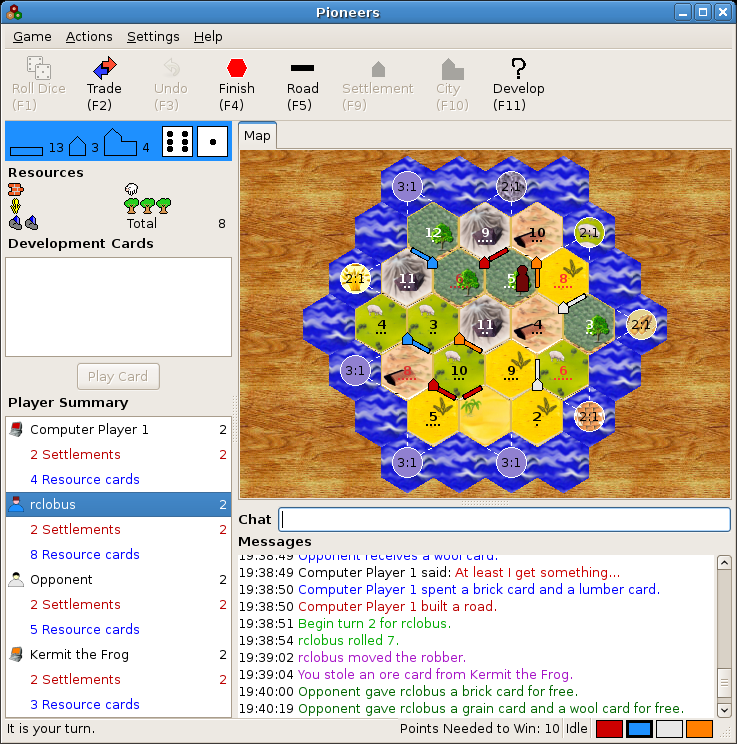
\includegraphics[width=\linewidth]{pioneers.png}
  \end{center}
  \caption{Zrzut ekranu z gry Pioneers}
  \label{pioneers}
\end{figure}

\subsection{JSettlers}
Aplikacja napisana w całości w Javie, rozwijana od początku 2004 roku
\cite{jsettlers}, dostępna na licencji GNU GPL. Aplikacja
przystosowana do uruchamiania w przeglądarce internetowej z
zainstalowanym środowiskiem uruchomieniowym Javy (\emph{ang. Java Runtime
  Environment}). Na \imref{jsettlers} został przedstawiony zrzut
ekranu z gry \emph{JSettlers}.

\begin{figure}[ht]
  \begin{center}
    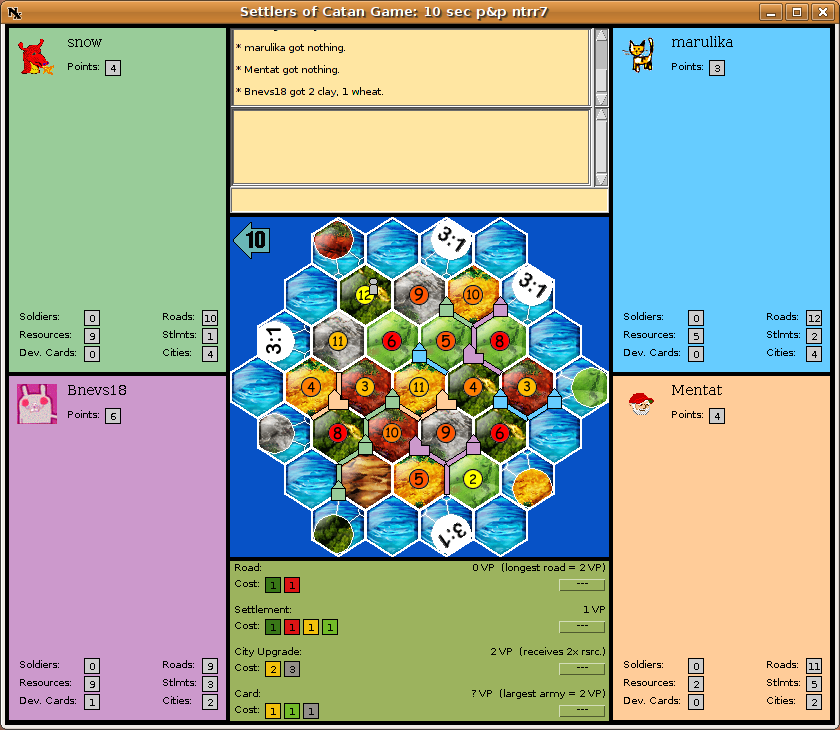
\includegraphics[width=\linewidth]{jsettlers.png}
  \end{center}
  \caption{Zrzut ekranu z gry JSettlers}
  \label{jsettlers}
\end{figure}

\subsection{Solito Server, MSN Games, PlayCatan.com}
Wszystkie te rozwiązania są oprogramowaniem własnościowym, w przypadku
dwóch ostatnich tytułów, płatnym. \emph{Solito Server} napisany został
przy użyciu technologii \emph{Adobe Flash}, dlatego jest w pewnym
stopniu uniezależniony od platformy sprzętowej (można go używać na
wszystkich platformach, na których dostępny jest \emph{Adobe
  Flash}). Pozostałe tytuły to oprogramowanie działające tylko i
wyłącznie pod kontrolą systemu operacyjnego \emph{Microsoft Windows},
wymagające instalacji.

\subsection{Catan - The First Island}
Jest to prawdopodobnie jedyna implementacja gry dedykowana urządzeniom
mobilnym. Pierwotnie aplikacja napisana została w Javie dla urządzeń
mobilnych, przez niemiecką firmę \emph{Exozet Games}. W połowie 2009
roku pojawiła się także wersja przeznaczona dla konsoli \emph{Nintendo
  DS}. Oba rozwiązania umożliwiają rozgrywkę z graczem komputerowym
(\emph{AI}), oraz z innymi graczami poprzez \emph{Bluetooth} lub
\emph{WiFi}. Nie posiadają one niestety żadnego centralnego
serwera. Obie opisywane wersje są płatnym oprogramowaniem
własnościowym.

\clearpage

\bibliographystyle{plain}
\bibliography{praca}

\end{document}
